\documentclass{article}
\usepackage[T1]{fontenc}

% Language setting
% Replace `english' with e.g. `spanish' to change the document language
\usepackage[spanish]{babel} % Manejo de idiomas
\usepackage[utf8]{inputenc}
% Set page size and margins
% Replace `letterpaper' with`a4paper' for UK/EU standard size
\usepackage[letterpaper,top=2cm,bottom=2cm,left=3cm,right=3cm,marginparwidth=1.75cm]{geometry}

% Useful packages
\usepackage{amsmath}
\usepackage{graphicx}
\usepackage{float}
\usepackage{times}
\usepackage{natbib}
\usepackage[colorlinks=true, allcolors=blue]{hyperref}
\spanishdecimal{.}
\usepackage{geometry}
\usepackage{graphics}
%\usepackage[sf,bf,tiny,center,compact]{titlesec}
\usepackage{subfigure}
\usepackage{tabularx}
\usepackage{amssymb}
\usepackage{mathrsfs}
\usepackage{hyphenat}
\usepackage{tikz}
\usepackage{blox}
\hyphenation{co-mer-cial rea-li-zan si-guien-te si-mu-la-ción ke-lly con-si-de-ra-da}
\bibpunct{(}{)}{;}{a}{,}{,}


\begin{document}

%portada
\begin{titlepage}
\centering
	\begin{figure}
  \begin{minipage}{1\linewidth}
     \centering\centering%\rule{2cm}{2cm}
    % \caption{Primera figura}
    
\includegraphics[width=0.3\textwidth]{img/logos_fi_uaq.png}
     
  \end{minipage}
\end{figure}
{\scshape\LARGE Universidad Autónoma de Querétaro \par}
	\vspace{0.5cm}
	{\scshape\Large Facultad de Ingeniería \par}
	\vspace{0.5cm}
	{\scshape\Large Ingeniería en Automatización \par}
	\vspace{0.5cm}	
	{\Large\bfseries Control III\par}
	\vspace{0.8cm}
	{\Large\bfseries Construcción, instrumentación y control de un Péndulo Invertido Sobre Dos Ruedas Seguidor de Línea (PISDRSL) \par}	
	\vspace{0.8cm}
	{\Large\itshape Primer entrega\par}
	\vspace{0.8cm}
	Profesor: \par
	Dr. Roberto Valentín Carrillo Serrano \par
	\vspace{0.5cm}
	Equipo 1\par \vspace{0.2cm}
	Integrantes:\vspace{0.4cm}\par	
	Aguilar Sarabia Diego Eugenio \rule{70mm}{0.1mm}
\vspace{0.4cm}
\par 
    Fernández Rendón Anna Patricia \rule{70mm}{0.1mm}
\vspace{0.4cm}
\par
	Sánchez Alejo Frida Alexandra \rule{70mm}{0.1mm}
\par
	
	\vfill

% Bottom of the page
	{\large Fecha compromiso: 5 de marzo del 2026\par
    Fecha en que se entregó: 28 de marzo del 2026}.
\end{titlepage}

%\frontmatter	%fija la numeración romana
\thispagestyle{empty}%no imprimir número de página en índice
\tableofcontents
\listoffigures
\listoftables
%\printindex
\newpage
%\setcounter{page}{1}
%\mainmatter 	%fija la numeración arábiga



\section{Objetivo}
Construir, instrumentar y controlar de manera embebida un robot de péndulo invertido sobre dos ruedas seguidor de línea (PISDRSL) que suba y baje pendientes de $15\ [^\circ]$

\section{Marco Teórico}
\subsection{Modelo no lineal del péndulo con dos ruedas}
\begin{figure} [H]
    \centering
    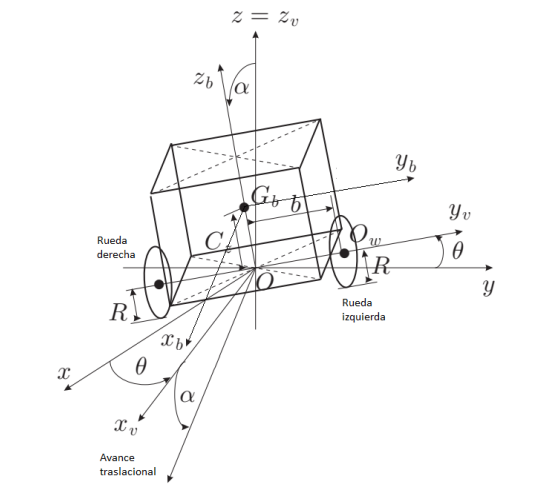
\includegraphics[width=0.77\linewidth]{img/Esquema_1.png}
    \caption{Péndulo con dos ruedas.}
    \label{fig:Esquema 1}
\end{figure}

El modelo dinámico no lineal del péndulo con dos ruedas obtenido con las ecuaciones de Euler-Lagrange está dado por \citep{HernandezBook2024}:

\begin{equation}
M(q)\ddot{q}+C(q,\dot{q})\dot{q}+g(q)=B(q)\tau
\label{eq:1}
\end{equation}

\begin{equation}
q=[x_o\quad y_o\quad \theta\quad \alpha\quad \phi_r\quad \phi_l]^T
\label{eq:2}
\end{equation}

\begin{equation}
M(q)=\begin{bmatrix}
M_p(1+\tan^2{(\beta)}) & 0 & \Delta_1 & \Delta_2 & 0 & 0\\ 
0 & M_p & \Delta_3 & \Delta_4 & 0 & 0\\
\Delta_1 & \Delta_3 & \Delta_5 & 0 & 0 & 0\\
\Delta_2 & \Delta_4 & 0 & M_pC_z^2+I_{yy} & 0 & 0\\
0 & 0 & 0 & 0 & M_wR^2+I_{wa} & 0\\
0 & 0 & 0 & 0 & 0 & M_wR^2+I_{wa}
\end{bmatrix}
\label{eq:3}
\end{equation}

\begin{equation}
\Delta_1=-M_pC_z\sin(\alpha)\sin(\theta)
\label{eq:4}
\end{equation}

\begin{equation}
    \Delta_2 = M_pC_z(\cos(\alpha)\cos(\theta)-\sin(\alpha)\tan(\beta))
    \label{eq:5}
\end{equation}

\begin{equation}
    \Delta_3=M_pC_z\sin(\alpha)\cos(\theta)
    \label{eq:6}
\end{equation}

\begin{equation}
    \Delta_4=M_pC_z\cos(\alpha)\sin(\theta)
    \label{eq:7}
\end{equation}

\begin{equation}
    \Delta_5=(M_pC_z^2+I_{xx})\sin^2(\alpha)+I_{zz}\cos^2(\alpha)+2I_{wd}
    \label{eq:8}
\end{equation}

\begin{equation}
    C(q,\dot{q})= \begin{bmatrix}
        0 & 0 & \Gamma_1 & \Gamma_2 & 0 & 0\\
        0 & 0 & \Gamma_3 & \Gamma_4 & 0 & 0\\
        0 & 0 & \Gamma_5 & \Gamma_6 & 0 & 0\\
        0 & 0 & -\Gamma_6 & 0 & 0 & 0\\
        0 & 0 & 0 & 0 & 0 & 0\\
        0 & 0 & 0 & 0 & 0 & 0\\
    \end{bmatrix}
    \label{eq:9}
\end{equation}

\begin{equation}
    \Gamma_1=-M_pC_z(\dot{\theta}\sin(\alpha)\cos(\theta)+\dot{\alpha}\sin(\theta)\cos(\alpha))
    \label{eq:10}
\end{equation}

\begin{equation}
    \Gamma_2=-M_pC_z(\dot{\theta}\sin(\theta)\cos(\alpha)+\dot{\alpha}\sin(\alpha)\cos(\theta)+\dot{\alpha}\cos(\alpha)\tan(\beta))
    \label{eq:11}
\end{equation}

\begin{equation}
    \Gamma_3=-M_pC_z(\dot{\theta}\sin(\alpha)\sin(\theta)-\dot{\alpha}\cos(\alpha)\cos(\theta))
    \label{eq:12}
\end{equation}

\begin{equation}
    \Gamma_4=M_pC_z(\dot{\theta}\cos(\alpha)\cos(\theta)-\dot{\alpha}\sin(\alpha)\sin(\theta))
    \label{eq:13}
\end{equation}

\begin{equation}
    \Gamma_5=(M_pC^2_z+I_{xx}-I_{zz})\dot{\alpha}\sin(\alpha)\cos(\alpha)
    \label{eq:14}
\end{equation}

\begin{equation}
    \Gamma_6=(M_pC^2_z+I_{xx}-I_{zz})\dot{\theta}\sin(\alpha)\cos(\alpha)
    \label{eq:15}
\end{equation}

\begin{equation}
    g(q)= \begin{bmatrix}
        (M_p+2M_w)g\tan(\beta) \\
        0 \\
        0 \\
        -M_pC_zg\sin(\alpha) \\
        0 \\
        0\\
    \end{bmatrix}
    \label{eq:16}
\end{equation}

\begin{equation}
    B(q)= \begin{bmatrix}
        0 & 0 \\
        0 & 0 \\
        0 & 0 \\
        -1 & -1 \\
        1 & 0 \\
        0 & 1\\
    \end{bmatrix}
    \label{eq:17}
\end{equation}

\begin{equation}
    \tau= \begin{bmatrix}
        \tau_r \\
        \tau_l \\
    \end{bmatrix}
    \label{eq:18}
\end{equation}
donde las coordenadas del punto $O$ son $(x_o,y_o)$, $\beta$ es el ángulo de una pendiente que sube el robot al avanzar, $R$ es el radio de la rueda, $g=9.81\;[\frac{m}{s^2}]$ es la aceleración de la gravedad, $M_p$ es la masa del péndulo, $C_z$ es la distancia del centro de masa del péndulo al punto $O$, $b$ es la distancia del punto $O$ al punto $O_w$, $I_{xx}$ es el momento de inercia calculado alrededor del eje $x_b$, $I_{yy}$ es el momento de inercia calculado alrededor del eje $y_b$, $I_{zz}$ es el momento de inercia calculado alrededor del eje $z_b$, $I_{wd}$ es el momento de inercia de la rueda alrededor de su diámetro, $I_{wa}$ es el momento de inercia de la rueda alrededor de su eje, $M_w$ es la masa completa de la rueda (llanta, rin, cople y rotor), $\phi_r$ es el ángulo de rotación de la rueda derecha, $\phi_l$ es el ángulo de rotación de la rueda izquierda, $\alpha$ es el ángulo de inclinación del péndulo, $\theta$ es el ángulo de orientación del robot y $v$ es la velocidad traslacional del robot dada como:
\begin{equation}
    v=\frac{R}{2}(\dot\phi_r+\dot\phi_l)
    \label{eq:19}
\end{equation}
La velocidad de orientación del péndulo con ruedas está dada por:
\begin{equation}
    \dot{\theta}=\frac{R}{2b}(\dot\phi_r-\dot\phi_l)
    \label{eq:20}
\end{equation}
\subsection{Modelo linealizado simplificado del péndulo con dos ruedas}
Cuando el robot realiza la tarea de seguidor de línea en una pista (línea de trayectoria deseada) las mediciones de las coordenadas $(x_o,y_o)$ del punto $O$ no son necesarias ya que esas variables se controlan indirectamente cuando la trayectoria deseada es seguida y esto mismo sucede con las posiciones de las ruedas del robot. Tomando ventaja de lo anteriormente descrito, es posible encontrar un modelo simplificado del robot.

Linealizando el modelo con restricciones no holonómicas del robot, asumiendo que $\beta=0$, $\alpha\approx0$ lo que implica $\cos(\alpha)\approx1$, $\sin(\alpha)\approx\alpha$ y definiendo $I_\phi$ como \citep{HernandezBook2024}:
\begin{equation}
    I_\phi=M_wR^2+I_{wa}
    \label{eq:21}
\end{equation}
se encuentra la aceleración traslacional del robot como:
\begin{equation}
    \boxed{I_\phi\dot{v}=\frac{R}{2}(\tau_r+\tau_l)}
    \label{eq:22}
\end{equation}
donde $\tau_r$ es el par aplicado a la rueda derecha y $\tau_l$ es el par aplicado a la rueda izquierda.

Linealizando el modelo en (\ref{eq:1}) se tiene \citep{HernandezBook2024}:
\begin{equation}
    \boxed{[d_5+I_\phi]\ddot{\theta}=\dfrac{R}{2b}(\tau_r-\tau_l)}
    \label{eq:23}
\end{equation}

\begin{equation}
    \boxed{\ddot{\alpha}-\dfrac{\sigma_1}{M_{22}}\alpha=-\sigma_2(\tau_r+\tau_l)}
    \label{eq:24}
\end{equation}

\begin{equation}
    d_5=I_{zz}+2I_{wd}
    \label{eq:25}
\end{equation}

\begin{equation}
    M_{22}=M_pC_z^2+I_{yy}
    \label{eq:26}
\end{equation}

\begin{equation}
    \sigma_1=gM_pC_z
    \label{eq:27}
\end{equation}

\begin{equation}
    \sigma_2=\dfrac{1}{M_{22}}\left[\dfrac{M_pC_zR}{2I_\phi}+1\right]
    \label{eq:28}
\end{equation} 

Así, el modelo linealizado simplificado del péndulo con dos ruedas está dado por las ecuaciones (\ref{eq:22}), (\ref{eq:23}) y (\ref{eq:24}).

\subsection{Controlador de seguimiento de línea}
Se define el controlador proporcional con retroalimentación de velocidad para seguimiento de línea (orientación del robot) de la siguiente manera \citep{HernandezBook2024}

\begin{equation}
    \boxed{\tau_a=\tau_r-\tau_l=\frac{2b}{R}\left[-k_v\dot{\theta}-k_p\tilde{\theta}\right], \quad \tilde{\theta}=\theta-\theta_d}
    \label{eq:29}
\end{equation}
donde $\theta_d$ es una constante y representa el valor deseado de la orientación del robot. Al sustituir (\ref{eq:29}) en (\ref{eq:23}) resulta:

\begin{equation}
    [d_5+I_\phi]\ddot{\theta}+k_v\dot{\theta}+k_p\theta=k_p\theta_d
    \label{eq:30}
\end{equation}

Así, si los coeficientes de sistema lineal de segundo orden en (\ref{eq:30}) son mayores que cero se asegura que $\dot{\theta}\rightarrow0$ y $\dot{\theta}\rightarrow\theta_d$ conforme transcurre el tiempo. Al aumentar $k_p$ se aumenta la rapidez en la respuesta y al aumentar $k_v$ se aumenta el amortiguamiento en la respuesta.

\subsection{Salida plana}
Ahora considere la siguiente función que es conocida como la salida plana \citep{HernandezBook2024}:

\begin{equation}
    \boxed{y_f=M_{22}\alpha+\sigma\int_0^t\tilde{v}(r)dr, \quad \sigma=M_pC_z+\frac{2}{R}I_\phi,\quad \tilde{v}=v-v_d}
    \label{eq:31}
\end{equation}
donde $v_d$ es una constante y representa el valor deseado de la velocidad traslacional de avance del robot. Diferenciando con respecto al tiempo tres veces consecutivas a (\ref{eq:31}) y sustituyendo expresiones algebraicas en el modelo (\ref{eq:22}), (\ref{eq:24}) y con las definiciones en (\ref{eq:28}) y (\ref{eq:31}) se puede llegar a \citep{HernandezBook2024}:

\begin{equation}
    \dot{y}_f=M_{22}\dot{\alpha}+\sigma\tilde{v}
    \label{eq:32}
\end{equation}

\begin{equation}
    \ddot{y}_f=\sigma_1\alpha
    \label{eq:33}
\end{equation}

\begin{equation}
    \dddot{y}_f=\sigma_1\dot{\alpha}
    \label{eq:34}
\end{equation}

\subsection{Controlador para balanceo y avance traslacional}
Empecemos definiendo el esfuerzo de control $u$ como sigue \citep{HernandezBook2024}:

\begin{equation}
    \boxed{u=\tau_r+\tau_l}
    \label{eq:35}
\end{equation}

Así usando (\ref{eq:24}), (\ref{eq:33}) y (\ref{eq:35}) se puede construir el diagrama de simulación analógica de la Figura \ref{fig:2}:

\begin{figure}[H]
    \centering
        \begin{tikzpicture}
            \bXInput{A}
            \bXBloc[2]{B}{$\sigma_2$}{A}
            \bXLink[$u$]{A}{B}
            \bXCompSum[4]{C}{B}{}{+}{-}{}
            \bXLink{B}{C}
            \bXBloc[2]{D}{$\int$}{C}
            \bXLink[$\ddot{\alpha}$]{C}{D}
            \bXBloc[2]{E}{$\int$}{D}
            \bXLink[$\dot{\alpha}$]{D}{E}
            \bXBloc[2]{F}{$\sigma_1$}{E}
            \bXLink[$\alpha$]{E}{F}
            \bXBloc[2]{G}{$\int$}{F}
            \bXLink[$\ddot{y}_f$]{F}{G}
            \bXBloc[2]{H}{$\int$}{G}
            \bXLink[$\dot{y}_f$]{G}{H}
            \bXOutput{I}{H}
            \bXLink[$y_f$]{H}{I}
            \bXBranchy[4]{F}{K}
            \bXBlocr[3.5]{L}{$\frac{1}{M_{22}}$}{K}
            \bXLinkyx{F-G}{L}
            \bXLinkxy{L}{C}
        \end{tikzpicture}
        \caption{Diagrama de simulación analógica de (\ref{eq:24}) y (\ref{eq:33}).}
        \label{fig:2}
    \end{figure}
    
Aplicando transformada de Laplace al diagrama de la Figura \ref{fig:2} se obtiene el diagrama de bloques siguiente \citep{HernandezBook2024}:

\begin{figure}[H]
    \centering
        \begin{tikzpicture}
            \bXInput{A}
            \bXBloc[3.5]{B}{$\sigma_2$}{A}
            \bXLink[$U(s)$]{A}{B}
            \bXCompSum[4]{C}{B}{}{+}{-}{}
            \bXLink{B}{C}
            \bXBloc[2]{D}{$\frac{1}{s}$}{C}
            \bXLink{C}{D}
            \bXBloc[2]{E}{$\frac{1}{s}$}{D}
            \bXLink{D}{E}
            \bXBloc[2]{F}{$\sigma_1$}{E}
            \bXLink{E}{F}
            \bXBloc[2]{G}{$\frac{1}{s}$}{F}
            \bXLink{F}{G}
            \bXBloc[2]{H}{$\frac{1}{s}$}{G}
            \bXLink {G}{H}
            \bXOutput[4]{I}{H}
            \bXLink[$Y_f(s)$]{H}{I}
            \bXBranchy[4]{F}{K}
            \bXBlocr[3.5]{L}{$\frac{1}{M_{22}}$}{K}
            \bXLinkyx{F-G}{L}
            \bXLinkxy{L}{C}
        \end{tikzpicture}
        \caption{Diagrama de bloques de la Figura \ref{fig:2}.}
        \label{fig:3}
    \end{figure}
    
Aplicando álgebra de bloques al diagrama de la Figura \ref{fig:3} se obtiene el siguiente diagrama de bloques simplificado:

\begin{figure}[H]
    \centering
        \begin{tikzpicture}
            \bXInput{A}
            \bXBloc[3.5]{B}{$\dfrac{-\sigma_1\sigma_2}{s^2-\dfrac{\sigma_1}{M_{22}}}$}{A}
            \bXLink[$U(s)$]{A}{B}
            \bXBloc[2]{C}{$\frac{1}{s^2}$}{B}
            \bXLink{B}{C}
            \bXOutput[4]{D}{C}
            \bXLink[$Y_f(s)$]{C}{D}
        \end{tikzpicture}
        \caption{Diagrama de bloques  simplificado de la Figura \ref{fig:3}.}
        \label{fig:4}
    \end{figure}
    
Dado que en la Figura \ref{fig:4} se tiene un sistema de cuarto orden, es posible asignar de manera arbitraria los cuatro polos de lazo cerrado si retroalimentamos $y_f$, $\dot{y}_f$, $\ddot{y}_f$ y $\dddot{y}_f$.  Esto se puede conseguir con el sistema en lazo cerrado de la Figura \ref{fig:5} \citep{HernandezBook2024}:

\begin{figure}[H]
    \centering
        \begin{tikzpicture}
            \bXInput{A}
            \bXCompSum[10]{B}{A}{}{+}{+}{}
            \bXLink[$R(s)=0$]{A}{B}
            \bXBloc[4]{C}{$\dfrac{-\sigma_1\sigma_2}{\left( s^2-\dfrac{\sigma_1}{M_{22}}\right)s^2}$}{B}
            \bXLink[$U(s)$]{B}{C}
            \bXOutput[10]{D}{C}
            \bXLink[$Y_f(s)$]{C}{D}
            \bXBranchy[5]{C}{K}
            \bXBlocr[-5]{L}{$k(s-z_1)(s-z_2)(s-z_3)$}{K}
            \bXLinkyx{C-D}{L}
            \bXLinkxy{L}{B}
        \end{tikzpicture}
        \caption{Diagrama de bloques del sistema en lazo cerrado.}
        \label{fig:5}
    \end{figure}
    
Debido a que los ceros están localizados en $z_1$, $z_2$ y $z_3$ en la ruta de retroalimentación de la Figura \ref{fig:5} lo que da como resultado la siguiente retroalimentación de estado \citep{HernandezBook2024}.

\begin{equation}
    U(s)=k(s-z_1)(s-z_2)(s-z_3)Y_f(s)
    \label{eq:36}
\end{equation}
que de manera polinomial está dada por:

\begin{equation}
    U(s)=k(s^3+a_2s^2+a_1s+a_0)Y_f(s)
    \label{eq:37}
\end{equation}
lo que implica:

\begin{equation}
    s^3+a_2s^2+a_1s+a_0=(s-z_1)(s-z_2)(s-z_3)
    \label{eq:38}
\end{equation}
y usando transformada inversa de Laplace se tiene que:

\begin{equation}
    u=k\:\dddot{y}_f+ka_2\ddot{y}_f+ka_1\dot{y}_f+ka_0y_f
    \label{eq:39}
\end{equation}
así sustituyendo (\ref{eq:31}), (\ref{eq:32}), (\ref{eq:33}) y (\ref{eq:34}) en (\ref{eq:39}) se obtiene:

\begin{equation}
    \boxed{u=k_1\dot{\alpha}+k_2\alpha+k_3\tilde{v}+k_4\int^t_0\tilde{v}(r)dr}
    \label{eq:40}
\end{equation}
donde:

\begin{equation}
    k_1=k(\sigma_1+a_1M_{22})
    \label{eq:41}
\end{equation}

\begin{equation}
    k_2=k(a_2\sigma_1+a_0M_{22})
    \label{eq:42}
\end{equation}

\begin{equation}
    k_3=ka_1\sigma 
    \label{eq:43}
\end{equation}

\begin{equation}
    k_4=ka_0\sigma 
    \label{eq:44}
\end{equation}

Una vez posicionados los ceros en $z_1$, $z_2$ y $z_3$ se puede encontrar el valor de $k$ mediante el diagrama de la Figura \ref{fig:6} con el lugar geométrico de las raíces que permita asignar los polos deseados de lazo cerrado:

\begin{figure}[H]
    \centering
        \begin{tikzpicture}
            \bXInput{A}
            \bXCompSum[10]{B}{A}{}{-}{+}{}
            \bXLink[$R(s)=0$]{A}{B}
            \bXBloc[4]{C}{$\dfrac{\sigma_1\sigma_2}{\left( s^2-\dfrac{\sigma_1}{M_{22}}\right)s^2}$}{B}
            \bXLink[$U_n(s)$]{B}{C}
            \bXOutput[10]{D}{C}
            \bXLink[$Y_f(s)$]{C}{D}
            \bXBranchy[5]{C}{K}
            \bXBlocr[-5]{L}{$k(s-z_1)(s-z_2)(s-z_3)$}{K}
            \bXLinkyx{C-D}{L}
            \bXLinkxy{L}{B}
        \end{tikzpicture}
        \caption{Diagrama de bloques del sistema en lazo cerrado con retroalimentación negativa, $U_n(s)=-U(s)$.}
        \label{fig:6}
    \end{figure}

\section{Materiales y Métodos}
\subsection{Materiales}
En el Cuadro \ref{tabla:materiales} se muestran los materiales empleados para el desarrollo de la práctica.  

\begin{table}[H]
\centering
\caption{Componentes electrónicos utilizados.} 
\begin{tabular}{|c|c|}\hline
Material: & Cantidad: \\ \hline
Micrcontrolador PIC18F4550 & 1\\
Amplificador operacional TL084 & 1\\
Potenciómetro $5\ [k\Omega]$ & 1\\
Capacitor cerámico $15\ [pF]$ & 2\\
Capacitor cerámico $0.1\,[\mu\text{F}]$ & 3\\
Capacitor cerámico $0.01\,[\mu\text{F}]$ & 1\\
Cristal de cuarzo $20\ [MHz]$ & 1\\
Resistencia $4.7\ [k\Omega]$ & 4\\
Resistencia $1\ [k\Omega]$ & 3\\
Resistencia $330\ [k\Omega]$ & 1\\
Resistencia $100\ [k\Omega]$ & 1\\
Resistencia $53\ [k\Omega]$ & 1\\
Micro switch 2 patas & 1\\
Alambre de cobre estañado calibre 22 de $1\ [m]$ & 1\\
\hline
\end{tabular}
\label{tabla:materiales}
\end{table}

En el Cuadro \ref{tabla:computadora} se muestra el equipo de cómputo utilizado para el desarrollo de la práctica.  

\begin{table}[H]
\centering
\caption{Equipo de cómputo utilizado.} 
\begin{tabular}{|c|c|}\hline
Características: & Descripción: \\ \hline
Fabricante & Acer\\
ID del dispositivo & 3C8E72CE-9F92-40F5-8A82-8D9E36929DB2 \\
Procesador & 11th Gen Intel(R) Core(TM) i7-11800H\\
Memoria RAM & 8 $[GB]$, procesador x64\\
Tipo de sistema operativo & Sistema operativo de 64 $[b]$, procesador x64\\
Especificaciones de Windows & 11 \textit{Home Single Language}
\\
\hline
\end{tabular}
\label{tabla:computadora}
\end{table}

En el Cuadro \ref{tabla:software} se muestran los software utilizados para el desarrollo de la práctica.  

\begin{table}[H]
\centering
\caption{El software empleado para el desarrollo de la práctica.} 
\begin{tabular}{|c|c|}\hline
Software: & Versión: \\ \hline
CCS Compiler & Versión 5.083\\
Proteus & Versión 8.15 \\
\hline
\end{tabular}
\label{tabla:software}
\end{table}

En el Cuadro \ref{tabla:materialLab} se muestra el equipo de laboratorio utilizado para el desarrollo de la práctica. 
\begin{table}[H]
\centering
\caption{El material del laboratorio empleado para el desarrollo de la práctica.} 
\begin{tabular}{|c|c|}\hline
Equipo: & Características: \\ \hline
Osciloscopio & Tektronix TDS2024B 4 canales, 200 $[MHz]$ de ancho de banda\\
Generador de funciones & Agilent 33210A \\
Fuente conmutada & Propiedad del docente \\
\hline
\end{tabular}
\label{tabla:materialLab}
\end{table}

\subsection{Diagrama de conexiones entre componentes}
\begin{figure}[H]
    \centering
    \includegraphics[width=0.5\textwidth]{img/Diagrama.jpg}
    \caption{Conexión eléctrica de los componentes de la práctica.}
    \label{fig:foto}
\end{figure}

\subsection{Metodología}
\subsubsection{Procedimiento}
La metodología utilizada para el desarrollo de la práctica se compone de diversas etapas:

\begin{enumerate}
\item Contrucción de prototipo físico de acuerdo con la Figura \ref{fig:foto} siguiendo todas las conexiones. 

\item Desarrollo de programa en CCS Compiler para poder leer una señal analógica y convertirla en una señal digital. 

\item Cálculos de el filtro que se utilizó para tener una señal más limpia. 

\item Configuramos la fuente dual con un voltaje de $\pm$ 12 $[V]$ para alimentar el amplificador operacional y +5V para alimentar el microcontrolador, además, en el osciloscopio configuramos los canales 1 y 2 con un acoplamiento de corriente continua (CC). Por último configuramos nuestros dos generadores de funciones, el primero va a ser el que va a introducir el ruido, va a tener una frecuencia de 10 $[Hz]$ y una amplitud de 3 $[V]$ y un offset de -2.5 $[V]$. El segundo osciloscopio se configuró con una amplitud de 2 $[V]$, sin offset y la frecuencia fue variable.

\item Pruebas con diferentes frecuencias para ver como se comporta el fenómeno de \textit{aliasing}. 

\end{enumerate} 

\subsubsection{Cálculos}
Se muestra el análisis de un filtro \textit{RC} de primer orden. La función de transferencia del sistema en el dominio de Laplace está dada por:

\begin{equation}
\frac{V_o(s)}{V_i(s)} = \frac{a}{s+a}
\end{equation}
donde:

\begin{equation}
a = \frac{1}{RC}
\end{equation}

La frecuencia angular de corte está definida como:

\begin{equation}
\omega_c = a = \frac{1}{RC}
\end{equation}
donde \textit{R} es la resistencia y \textit{C} es el capacitor, esto se relaciona con la frecuencia de corte en Hertz mediante:

\begin{equation}
\omega_c = 2\pi f_c
\end{equation}

Para una frecuencia de corte deseada tal que:

\begin{equation}
\omega_c = 188.49 \, \text{rad/s}
\end{equation}
y considerando un capacitor de:

\begin{equation}
C = 0.1 \, \mu F
\end{equation}
se despeja el valor de la resistencia:

\begin{equation}
R = \frac{1}{\omega_c C}
\end{equation}

Sustituyendo valores:

\begin{equation}
R = \frac{1}{(188.49)(0.1 \times 10^{-6})}
\end{equation}
obteniéndose:

\begin{equation}
R = 53 \, k\Omega
\end{equation}

Dado que se selecciona el valor comercial más cercano, se emplea una resistencia de:

\begin{equation}
R = 51 \, k\Omega
\end{equation}

Con este valor comercial, la nueva frecuencia angular de corte es:

\begin{equation}
\omega_c = \frac{1}{RC} = 196.07 \, \left[\frac{\text{rad}}{\text{s}}\right]
\end{equation}
y por lo tanto, la frecuencia de corte real resulta:

\begin{equation}
f_c = 31.2 \, [Hz]
\end{equation}

\section{Resultados y Discusión}
\begin{figure}[H]
    \centering
    \includegraphics[width=0.5\textwidth]{img/45Hz - Esquema_1.png}
    \caption{Imagen de oscilocopio con un muestreo de 10 $[ms]$ y la señal tiene una frecuencia de 45 $[Hz]$ sin filtro.}
    \label{fig:Esquema_1}
\end{figure}




\subsection{Aguilar Sarabia Diego Eugenio}
En esta práctica se analizó la importancia del filtrado previo a la etapa de conversión analógico-digital para mitigar el fenómeno de \textit{aliasing}. Al observar los resultados experimentales en el osciloscopio, se identificó que la señal senoidal presentaba componentes de alta frecuencia (ruido) que distorsionaban la información original. Para solucionar esto, se diseñó un filtro RC de primer orden con una frecuencia de corte teórica de 30 $[Hz]$. Debido a la disponibilidad de componentes, se empleó una resistencia comercial de $51\ [k\Omega]$, lo que ajustó la frecuencia de corte real a 31.2 $[Hz]$. Esta implementación permitió que el microcontrolador PIC18F4550 procesara una señal más limpia, cumpliendo con el objetivo de adquirir datos de manera fiel al limitar el ancho de banda de entrada conforme a los criterios de muestreo.

\subsection{Alanis Martínez Jose Jeancarlo}
Durante el desarrollo de la práctica se pudo analizar de forma experimental 
cómo influye el periodo de muestreo en la calidad de la señal digitalizada 
y posteriormente reconstruida. Se trabajó con una señal analógica conformada 
por una componente principal y ruido, la cual fue aplicada al convertidor 
analógico-digital del microcontrolador PIC18F4550. Posteriormente, la señal 
fue reconstruida mediante un convertidor digital-analógico, permitiendo 
observar directamente los efectos del muestreo.

Se comprobó que el parámetro determinante fue la frecuencia de muestreo 
($f_s$), la cual está directamente relacionada con el periodo de muestreo 
($T_s$) y define la frecuencia de Nyquist 
($f_N = \frac{f_s}{2}$). 
Cuando la frecuencia de la señal de entrada se mantuvo por debajo de dicho 
límite, la forma de onda obtenida a la salida del \textit{DAC} presentó 
una alta similitud con la señal original, sin deformaciones apreciables.

Por ejemplo, al emplear un periodo de muestreo de 
$1\,[\mathit{ms}]$ ($f_s = 1000\,[\mathit{Hz}]$), 
el sistema logró reconstruir correctamente señales con frecuencias 
inferiores a $500\,[\mathit{Hz}]$. En estas condiciones, el microcontrolador 
capturó suficientes muestras por cada ciclo, lo que permitió representar 
adecuadamente la información contenida en la señal y reproducirla con fidelidad. 
De manera similar, cuando se utilizó un periodo de 
$10\,[\mathit{ms}]$ ($f_s = 100\,[\mathit{Hz}]$), 
la reconstrucción adecuada solo fue posible para frecuencias menores 
a $50\,[\mathit{Hz}]$.

Al incrementar la frecuencia de la señal por encima de la frecuencia de 
Nyquist correspondiente, comenzaron a observarse alteraciones importantes 
en la señal reconstruida. Estas modificaciones se manifestaron como cambios 
en la forma y en la frecuencia aparente de la señal de salida. La causa de 
este comportamiento fue la reducción en el número de muestras por ciclo, 
lo cual impidió que el \textit{ADC} capturara información suficiente para 
describir correctamente la señal original.

Este efecto corresponde al fenómeno de \textit{aliasing}, donde componentes 
de frecuencia superiores al límite permitido se reflejan dentro del rango 
válido del sistema, generando frecuencias falsas o distorsionadas en la 
señal digitalizada. En consecuencia, el \textit{DAC} reproduce una forma 
de onda que no representa con exactitud la señal aplicada inicialmente.

Como medida preventiva, se identificó la importancia de implementar un 
filtro pasabajas previo al proceso de muestreo. Este filtro, conocido como 
filtro \textit{antialiasing}, limita el contenido espectral de la señal 
a valores menores que la frecuencia de Nyquist, eliminando o atenuando 
las componentes que podrían provocar \textit{aliasing}. De esta manera, 
se garantiza que el sistema de adquisición procese únicamente información 
que pueda ser correctamente muestreada y reconstruida.

En conclusión, la práctica permitió verificar experimentalmente que la 
selección adecuada de la frecuencia de muestreo es un factor crítico en 
los sistemas digitales de adquisición. Un valor insuficiente de $f_s$ 
compromete la integridad de la señal y genera distorsiones, mientras que 
un muestreo correctamente definido preserva la fidelidad de la información 
durante todo el proceso de digitalización y reconstrucción.

\subsection{Fernández Rendón Anna Patricia}
Se realizaron varios  

\subsection{Loredo Guillén Ulises Hiram}
Con los resultados obtenidos durante la práctica, se pudo constatar 
de forma experimental los efectos del fenómeno de muestreo sobre 
una señal senoidal contaminada por ruido.  

Cuando se elevó la frecuencia de muestreo a un valor por encima del 
doble de la frecuencia máxima de la señal, la forma de onda digital 
obtenida se vio mejorada. Se observó que la representación discreta 
conservaba mejor la amplitud y la frecuencia de la señal analógica, 
lo que valida experimentalmente el criterio de Nyquist.  

Los resultados obtenidos con el filtro \textit{anti-aliasing} 
mostraron una reducción considerable del ruido de alto rango de 
frecuencias en la señal de entrada. Sin el filtro, las muestras 
presentaban una mayor dispersión y se percibían variaciones en la señal. 
Con el filtro, la señal digital obtenida es más estable y se asemeja 
más a la forma de onda senoidal original. Por lo tanto, los resultados 
experimentales coinciden con los fundamentos teóricos estudiados 
previamente, en particular con el fenómeno de \textit{aliasing}.

\subsection{Luna Loarca Raúl}
El comportamiento observado dependió directamente del periodo de muestreo 
$T_s$ seleccionado. Para un periodo de muestreo de 
$1\,[\textit{ms}]$, equivalente a una frecuencia de muestreo de 
$1\,[\textit{kHz}]$, la señal pudo reconstruirse correctamente cuando la 
frecuencia de la señal de entrada era menor a $500\,[\textit{Hz}]$. 
Este resultado coincide con el criterio de Nyquist, el cual establece 
que la frecuencia de muestreo debe ser al menos el doble de la frecuencia 
máxima presente en la señal para evitar la pérdida de información.

Por debajo de este límite, el microcontrolador fue capaz de capturar 
suficientes muestras por periodo de la señal, permitiendo que el DAC 
reconstruyera una forma de onda similar a la señal original.

Sin embargo, cuando la frecuencia de la señal de entrada superó los 
$500\,[\textit{Hz}]$, comenzaron a observarse distorsiones significativas 
en la señal reconstruida. Estas distorsiones se debieron directamente al 
fenómeno de \textit{aliasing}. Al no cumplirse el criterio de Nyquist, el 
sistema tomó un número insuficiente de muestras por ciclo de la señal, 
lo que provocó que el microcontrolador interpretara la señal como si 
tuviera una frecuencia diferente. Como resultado, la señal reconstruida 
presentó deformaciones y pérdida de fidelidad respecto a la señal original.

Cuando se utilizó un periodo de muestreo mayor, como 
$10\,[\textit{ms}]$, el límite de Nyquist se redujo a 
$50\,[\textit{Hz}]$, por lo que el \textit{aliasing} ocurrió a frecuencias 
mucho más bajas.

Se demostró que el \textit{aliasing} es un fenómeno inherente a los sistemas 
de adquisición digital cuando la frecuencia de muestreo no es suficientemente 
alta. La práctica permitió comprobar que la correcta selección de la 
frecuencia de muestreo es fundamental para conservar intacta la señal y 
evitar la aparición de distorsiones en el proceso de reconstrucción.

Durante la práctica se observó experimentalmente el fenómeno de 
\textit{aliasing} al muestrear una señal analógica compuesta por una señal 
portadora y una señal de ruido, la cual fue introducida al ADC del 
microcontrolador PIC18F4550 y posteriormente reconstruida mediante un DAC. 
El comportamiento del sistema dependió directamente del periodo de muestreo 
$T_s$ y, por lo tanto, de la frecuencia de muestreo $f_s$ y su correspondiente 
frecuencia de Nyquist $f_N = \frac{f_s}{2}$.

Se comprobó que cuando la frecuencia de la señal de entrada se mantuvo 
por debajo de la frecuencia de Nyquist, la señal reconstruida por el DAC 
conservó su forma original, sin presentar distorsiones ni pérdidas 
apreciables. En el caso de un periodo de muestreo de 
$10\,[\textit{ms}]$, las señales con frecuencia menor a 
$50\,[\textit{Hz}]$ pudieron reconstruirse correctamente. De igual forma, 
con un periodo de muestreo de $1\,[\textit{ms}]$, las señales con 
frecuencia menor a $500\,[\textit{Hz}]$ también fueron reconstruidas con 
fidelidad. Esto se debe a que el microcontrolador fue capaz de adquirir un 
número suficiente de muestras por ciclo, permitiendo representar de manera 
adecuada la información de la señal y reproducirla correctamente mediante 
el DAC.

En contraste, cuando la frecuencia de la señal de entrada fue mayor que la 
frecuencia de Nyquist, es decir, superior a $50\,[\textit{Hz}]$ para 
$T_s = 10\,[\textit{ms}]$ y superior a $500\,[\textit{Hz}]$ para 
$T_s = 1\,[\textit{ms}]$, la señal de salida comenzó a presentar distorsiones 
y deformaciones visibles. Esto ocurrió porque el microcontrolador no pudo 
recopilar la cantidad de muestras necesarias para describir correctamente 
cada ciclo de la señal. Como consecuencia, los valores digitales obtenidos 
por el ADC no representaron la señal original, y el DAC reconstruyó una 
señal incorrecta, con cambios en su forma y frecuencia. Este comportamiento 
corresponde directamente al fenómeno de \textit{aliasing}.

Asimismo, se identificó que una solución para evitar este problema consiste 
en utilizar un filtro pasabajas \textit{antialiasing} antes de la etapa de 
muestreo. Este filtro permite el paso únicamente de las frecuencias menores 
a la frecuencia de Nyquist y atenúa o elimina las componentes de mayor 
frecuencia que no pueden ser correctamente muestreadas. De esta forma, se 
garantiza que el microcontrolador procese información válida y que el DAC 
reconstruya la señal sin distorsiones.

En general, los resultados obtenidos permitieron comprobar de forma práctica 
la relación directa entre la frecuencia de muestreo y la fidelidad de la 
señal reconstruida, así como la importancia del uso de filtros adecuados 
para prevenir el \textit{aliasing} en sistemas de adquisición de datos 
digitales.

\subsection{Sánchez Alejo Frida Alexandra}
Al analizar el desempeño del sistema de adquisición con el microcontrolador 
PIC18F4550, es notable la cercanía entre los datos de simulación y los 
experimentales. En Proteus, se observó un tiempo de levantamiento 
($t_r$) de $0.08454\,[\textit{s}]$ y un sobrepaso ($M_p$) de 
$76.92\,[\%]$. En contraste, las mediciones físicas mostraron un 
$t_r$ de $0.08431\,[\textit{s}]$ y un $M_p$ de $76.98\,[\%]$.

Esta mínima discrepancia indica que el circuito fue armado con alta 
fidelidad respecto al diseño original. La decisión de utilizar una 
resistencia comercial de $51\,\text{k}\Omega$ en lugar de la teórica 
de $53\,\text{k}\Omega$ ajustó la frecuencia de corte a 
$31.2\,[\textit{Hz}]$, un valor que resultó ser sumamente efectivo 
para proteger la señal de distorsiones por \textit{aliasing}.               
 
\subsection{Resultados y discusión del equipo}
Para el desarrollo de esta práctica, se comprobó de forma experimental qué es y cómo se comporta el fenómeno de \textit{aliasing}. A lo largo de todas las figuras, se puede observar que, a frecuencias menores que la frecuencia de Nyquist, la señal reconstruida puede distorsionarse, así como representarse de manera incorrecta, lo cual confirma la teoría de muestreo. 

Sin embargo, este fenómeno puede mitigarse si se emplea un filtro \textit{antialiasing}. Para esta práctica se utilizó un filtro RC de primer orden que, al ser calculado correctamente, permitió reducir los efectos del \textit{aliasing}. 

Cuando no se utilizaba el filtro, la señal presentaba distorsiones en su forma, asimetría e incluso saturación. Al implementar el filtro, se pudo observar una señal mucho más limpia y simétrica con respecto a la señal original.



\section{Conclusiones}
\subsection{Aguilar Sarabia Diego Eugenio}
Concluyo que el diseño e implementación de un filtro \textit{antialiasing} es un elemento determinante para garantizar la integridad de los datos en sistemas de adquisición digitales. A través de la experimentación, se comprobó que el uso de herramientas de desarrollo como CCS Compiler y Proteus permite validar el comportamiento del \textit{firmware} en el microcontrolador, pero es el acondicionamiento físico de la señal (el filtro analógico) lo que evita errores de reconstrucción irreversibles. El proyecto demostró con éxito que, al mantener las frecuencias de entrada por debajo del límite de corte diseñado, se obtiene una representación digital estable y funcional para aplicaciones de control.
 

\subsection{Alanis Martínez Jose Jeancarlo}
El propósito de la práctica se alcanzó al diseñar y poner en funcionamiento un sistema de adquisición de datos utilizando el microcontrolador PIC18F4550. Con este sistema fue posible tomar muestras de una señal senoidal que presentaba ruido, lo que permitió analizar su comportamiento durante el proceso de digitalización. A lo largo del desarrollo se pudo reconocer cómo se presenta el fenómeno aliasing y entender por qué el límite de Nyquist es un punto clave al momento de definir la frecuencia de muestreo.
Al incorporar un filtro antialiasing antes del proceso de conversión, se observó una mejora en la señal obtenida. Este filtro ayudó a reducir las alteraciones causadas por componentes no deseados, permitiendo conservar mejor la información importante de la señal original y obtener datos digitales de mayor calidad.

\subsection{Fernández Rendón Anna Patricia}
En esta práctica conocimos el fenómeno \textit{aliasing} que se presenta cuando la frecuencia de muestreo está por debajo de la frecuencia de Nyquist. Al no muestrar correctamente la señal, se tienen puntos insuficientes para replicar la señal deseada. Como pudimos observar en los resultados, cuando estábamos por debajo de la frecuencia de Nyquist, la señal tenia puntos que no correpondian a la señal original o incluso no alcanzaba a apreciarse la forma senoidal que debería pero también juega un papel muy impoprtante el hecho de agregar un filtro; en este caso fue un filtro RC de primer orden que permitió filtrar la señal y así obtener mejores resultados. Además, jugar con la parte de la frecuencia de la señal nos permitió ver el fenómeno de \textit{aliasing} en su máximo esplendor, ya que en cuando se tenía un tiempo de muestreo de 1 $[ms]$ y una frecuencia de 950 $[ms]$ y sin el filtro implementado, se podía observar el fenómeno de \textit{aliasing} en su máximo esplendor al ver la señal de salida del DAC con mucha saturación, nada simétrica y con mucha distorsión. Este tipo de fenómenos son importantes conocerlos ya que se pueden presentar en muchos ámbitos laborales y es importante saber cómo solucionarlos, con un filtro RC muy bien calculado es fácil poder corregirlo. 

\subsection{Loredo Guillén Ulises Hiram}
En esta práctica se llevó a cabo la construcción e implementación 
de un sistema de adquisición de datos basado en el microcontrolador 
PIC18F4550, el cual se utilizó para analizar de manera experimental 
el proceso de muestreo de una señal senoidal contaminada con ruido. 
Fue necesario establecer una frecuencia de muestreo adecuada para 
evitar la distorsión de la señal original.

Además, la inclusión de un filtro \textit{antialiasing} en la entrada 
del ADC demostró ser una etapa fundamental del sistema, con el objetivo 
de limitar el contenido en frecuencia de la señal y así prevenir el 
fenómeno de \textit{aliasing}. Debido a esto, se mejoró la calidad de 
las muestras obtenidas y se logró una representación digital más cercana 
a la señal analógica original.

En conjunto, el desarrollo de esta práctica no solo reforzó el criterio 
de Nyquist como condición ineludible en los sistemas de muestreo, sino 
que también permitió comprender la importancia del acondicionamiento 
de la señal en sistemas embebidos.
 
\subsection{Luna Loarca Raúl}
A partir de la implementación práctica con el microcontrolador 
PIC18F4550, se comprobó que el fenómeno de \textit{aliasing} es una 
consecuencia directa de un muestreo insuficiente en relación con la 
frecuencia de la señal de entrada. Se observó que cuando la frecuencia 
de muestreo fue de $1\,[\textit{kHz}]$, la señal pudo reconstruirse 
correctamente únicamente para frecuencias menores a $500\,[\textit{Hz}]$, 
lo cual coincide con el criterio de Nyquist, confirmando que la 
frecuencia de muestreo debe ser al menos el doble de la frecuencia 
máxima de la señal para preservar su forma original.

Asimismo, se verificó que al superar la frecuencia de Nyquist, el 
microcontrolador no pudo adquirir suficientes muestras por ciclo, 
lo que provocó una reconstrucción incorrecta mediante el DAC. 
Esto se manifestó en forma de distorsión, evidenciando la pérdida 
de información causada por el \textit{aliasing}. Este resultado 
permitió comprender que el sistema digital interpreta la señal de 
manera incorrecta debido a la limitación impuesta por la frecuencia 
de muestreo.

En general, la práctica permitió la comprensión del fenómeno 
\textit{aliasing}, destacando la importancia de la frecuencia de 
muestreo y del acondicionamiento de la señal para garantizar una 
reconstrucción fiel en sistemas digitales de control.
 
\subsection{Sánchez Alejo Frida Alexandra}
En esta práctica, pude comprobar que un buen código en CCS Compiler 
no es suficiente si el circuito físico no está bien diseñado y ensamblado. 
La construcción del prototipo siguiendo el diagrama de conexiones fue 
fundamental para que el PIC18F4550 procesara la señal correctamente. 
Al implementar el filtro \textit{antialiasing} con una frecuencia de 
corte real de $31.2\,[\textit{Hz}]$, logramos proteger la integridad 
de la señal senoidal frente al ruido y las frecuencias no deseadas. 

Ver que el sobrepaso experimental fue casi idéntico al de la simulación 
me confirma que un diseño de hardware robusto es la base necesaria para 
que cualquier sistema de adquisición de datos sea confiable.
 
\subsection{Conclusiones del equipo}
Pudimos identificar qué es el fenómeno de \textit{aliasing} y qué puede ocurrir si se trabaja por debajo de la frecuencia de Nyquist, teniendo pérdidas de información en la señal, lo cual resulta perjudicial, ya que pueden obtenerse datos que no correspondan a los originales. En este caso, esto provocó que la señal no fuera completamente senoidal, sino asimétrica y distorsionada. 

Por ello, se remarca la importancia de implementar un filtro \textit{antialiasing}, cuyos cálculos sean lo más precisos posible para garantizar su correcto funcionamiento. 

Además, se presentó un reto importante durante el armado del circuito, ya que en las primeras dos ocasiones la placa donde se realizaba el montaje generaba falsos contactos, lo que provocaba errores graves que ya no dependían directamente de la programación ni del filtro implementado.


\vspace{10 mm}
\addcontentsline{toc}{section}{Bibliografía}
\bibliographystyle{uaq_prev}%{uaq_prev}%{apalike}%{apsr}%{apalike}%{abbrvnat}%archivo .bst
\bibliography{rep}%archivo .bib

\newpage
\section{Anexos}

\subsection{Programa en CSS compiler para reconstruir la señal filtrada}\label{proggsim}
En este anexo se muestra el código fuente de CCS compiler para ver como el microcontrolador recontruia la señal con aliasing y sin aliasing a diferentes frecuencias. 
{\scriptsize
\begin{verbatim}
#include <18F4550.h>
#DEVICE ADC=8
#include <stdlib.h>
#include <stdio.h>
#include <math.h>
#FUSES NOWDT //No Watch Dog Timer
#FUSES NOPROTECT //No Watch Dog Timer
#FUSES NOBROWNOUT //No brownout reset
#FUSES NOLVP //No low voltage prgming, B3(PIC16) or B5(PIC18) used for I/O
#FUSES HS
#use delay (clock = 20M, crystal = 20M) 
//direcciones de los puertos
#byte porta = 0xf80
#byte portb = 0xf81
#byte portc = 0xf82
#byte portd = 0xf83
#byte porte = 0xf84
#bit PC0 = 0xf82.0 //
#bit PC1 = 0xf82.1
// Registros del Timer
#byte TMR0L = 0xfd6 //TMR0L
#byte T0CON = 0xfd5 //T0CON
#byte INTCON= 0xff2 //INTCON

//Define de las pendientes 
#define mi 0.019607
#define mo 25.5


int8 tope=196, cuenta=0;
float vi = 0.0, vo = 0.0; 
 
void main (void)
{
   setup_adc_ports(ALL_ANALOG);
   setup_adc(ADC_CLOCK_INTERNAL); 
   set_adc_channel(0); 
   delay_us(10); 
   
   //set_tris_a(0b11111111);
   set_tris_b(0b11111111);
   set_tris_c(0b11111110);    
   set_tris_d(0b00000000);
   set_tris_e(0b11111111);
   
   T0CON=0xC7; //Prescaler asignado a timer0 con relación 1:256
   TMR0L=0;   
   while(true)
   {
      //PORTD = read_adc();
      
      vi = mi * read_adc(); 
      
      vo=vi;
      
      PORTD=mo*vo+127.0;
      
      while (TMR0L<=tope)
      {
         if(PC1) 
            tope=196;
         else 
            tope=20;
         PC0 =0;
      }
      PC0=1;
      TMR0L=0;
   }
}
\end{verbatim}
}
\end{document}